% % % % % % %
%  Packages %
% % % % % % %

%---Base packages
\documentclass[a4paper,12pt]{report}	% document type (article, report, book)
\usepackage[utf8]{inputenc}			% encoding
\usepackage[T1]{fontenc}			% accent
\usepackage{lmodern}				% latin font
\usepackage{appendix}				% to be able to use appendices
\usepackage{float,graphicx}	
\usepackage{algorithm}
\usepackage{algorithmic}	

%---Language(s)
\usepackage[english,frenchb]{babel}	% last language = typography by default
\addto\captionsfrench{				% to change the french names of...
	\renewcommand{\appendixpagename}{Annexes}	% (default Appendices)
	\renewcommand{\appendixtocname}{Annexes}	% (default Appendices)
	\renewcommand{\tablename}{\textsc{Tableau}}	% (default \textsc{Table})
}

%---Page layout
%------> margins
	% 1st option -> geometry package
		%\usepackage[a4paper]{geometry}		% default parameters for A4
		%\usepackage[top=2in, bottom=1.5in, left=1in, right=1in]{geometry}
	% 2nd option -> a4wide package
		\usepackage{a4wide}		% A4 with smaller margins (the one I've chosen)
	% 3rd option -> fullpage package
		%\usepackage{fullpage}
%------> chapter style
	% 1st option -> fncychap package
		%\usepackage[style]{fncychap}		% style = Lenny, Bjornstrup, Sonny, Conny
	% 2nd option -> customized styles
		%
%------> cover page (UMONS template)
	\usepackage[fs]{umons-coverpage}		% NEED "umons-coverpage.sty" file
	\umonsAuthor{Réalisé par Louis \textsc{Dascotte} \\ \& Nicolas \textsc{Delplanque} \\ \& Nicolas \textsc{Sournac} } 
	\umonsTitle{Traitement du signal : Projet}
	\umonsSubtitle{Speaker classification}
	\umonsDocumentType{I-ISIA-030}
	\umonsDate{3e Bachelier en Sciences Informatiques\\ Année 2021-2022}

%---Numbering
\setcounter{secnumdepth}{2}			% numerotation depth (1=sec and all above)
\setcounter{tocdepth}{2}			% table of contents depth (1=sec and above)

%---Mathematics
\usepackage{amsmath}				% base package for mathematics
\usepackage{amsfonts}				% base package for mathematics
\usepackage{amssymb}				% base package for mathematics
%\usepackage{amsthm}				% theorem and proof environments
%\usepackage{cases}					% numcases environment
%\usepackage{mathrsfs}				% \mathscf command ('L' of Laplace-Transform,...)

%---Floating objects (images, tables,...)
\usepackage{float}					% better management of floating objects
\usepackage{array}					% better management of tables
\usepackage{graphicx}				% to include external images
\graphicspath{{Images/}}			% to put images in an 'Images' folder 
%\usepackage{caption}				% /!\ has priority on "memoir" class
%\usepackage{subcaption}			% subfigure and subtable environments
%\usepackage{subfig}				% \subfloat command
%\usepackage{wrapfig}				% wrapfigure environment
%\usepackage[update]{epstopdf}		% to use '.eps' files with PDFLaTeX

\setlength{\extrarowheight}{.5ex}


%---Units from International System
\usepackage{siunitx}				% \SI{}{} command (units with good typography)
\DeclareSIUnit\baud{baud}			% definition of the "baud" unit
\DeclareSIUnit\bit{bit}				% definition of the "bit" unit

%---Drawing
%\usepackage{tikz}					% useful package for drawing
%\usepackage[european]{circuitikz} 	% to draw electrical circuits

%---Bibliography
\usepackage{url}					% to encore url
\usepackage[style=numeric-comp,backend=bibtex]{biblatex}
\usepackage{csquotes}				% inverted commas in references
%\bibliography{bibli}				% your .bib file

%---"hyperref" package				% /!\ it must be the last package
\usepackage[hidelinks]{hyperref}	% clickable links (table of contents,...)


\newcommand*{\addheight}[2][.5ex]{%
	\raisebox{0pt}[\dimexpr\height+(#1)\relax]{#2}%
}

% % % % % % %
% Document	%
% % % % % % %

\begin{document}

\umonsCoverPage		% produce the cover page with UMONS and your Faculty logo
	
\pagenumbering{roman}	% if you don't use the class "book"

\begin{abstract}
Ce rapport contient l'ensemble des résultats obtenus, leurs interprétations ainsi que les explications du fonctionnement de notre implémentation du projet de traitement du signal. Ce projet consiste en la réalisation de solutions visant à classifier des personnes en fonction de leur genre à partir d'enregistrement de leur voix.
\end{abstract}

\clearpage		
\tableofcontents

\clearpage		
\pagenumbering{arabic}

{\section*{1. Exécution du code}}
\addcontentsline{toc}{chapter}{1. Exécution du code/ Structure}
Le fichier main.py doit être lancé depuis la racine du projet. Il en est de même pour les fichier utils.py et ml\_utils.py, il faut alors exécuter les commandes : "python src/main/utils.py" et "python src/main/ml\_utils.py". Les fichiers tests doivent quant à eux être exécuté depuis le dossier où ils sont stockés.
{\subsection*{1.1 Librairies utilisées}}
\addcontentsline{toc}{section}{1.1 Librairies utilisées}
Afin de réaliser ce projet, nous avons été amenés à utiliser des librairies extérieures aux librairies de bases que nous proposait python :\\
- audiofile : permet d'extraire le signal et la fréquence d'échantillonnage des fichiers audios.\\
- numpy (version 1.20) : utilisée pour les différentes fonctions mathématiques. \\
- scipy : utilisée pour avoir le signal et les transformées de Fourier. \\
-pickle : utiliser pour sauvegarder et charger des objets. \\
-pandas : utiliser pour lire les CSV .\\
-torch : utiliser pour instancier le modèle de machine learning et le paramétrer. \\
-sklearn : utiliser pour instancier le scaler. \\
{\subsection*{1.2 Structure du code source}}
\addcontentsline{toc}{section}{1.2 Structure du code source}
Le projet est divisé en plusieurs dossiers. Le dossier racine contient un dossier data contenant l'ensemble des fichiers audio utilisés lors de la réalisation du projet ainsi que les données relatives au modèle de machine learning, et un dossier src contenant la source du programme (ce qui est utilisé par le programme en lui-même ainsi que les tests unitaires).

{\section*{2. Caractéristiques étudiées}}
	\addcontentsline{toc}{chapter}{2. Caractéristiques étudiées}
Pour la réalisation du projet, nous avons été amenés à étudier différentes caractéristiques des signaux de parole en vue de les utiliser afin de pouvoir classifier les différents speakers. Pour chacune de ces caractéristiques, nous avons donc implémenté un algorithme qui permet de la calculer et nous avons ensuite analysé et interprété ses résultats afin d'en déduire les règles sur lesquelles la classification se base.

{\subsection*{2.1 Energie du signal}}
\addcontentsline{toc}{section}{2.1 Energie du signal}
L'énergie du signal est calculée à partir de la fonction compute\_energy() qui prend un signal en paramètre. Cette fonctionne parcourt simplement l'entièreté du signal en question et y applique la formule du calcul de l'énergie. Nous utilisons les résultats du calcule de l'énergie du signal afin de déterminer si une frame est voiced ou unvoiced.
{\subsection*{2.2 Fréquence fondamentale}}
\addcontentsline{toc}{section}{2.2 Fréquence fondamentale}
Le pitch ou la fréquence fondamentale représente la plus basse fréquence qui constitue un signal. Cette valeur doit varier entre 60 Hz pour les voix les plus graves et 550 Hz pour les voix les plus aigües. \\
Lors du projet, nous avons été amenés à calculer la fréquence fondamentale des speakers en utilisant deux méthodes différentes : La méthode basée sur l'autocorrelation et la méthode basée sur les cepstrums. Pour ce faire, nous avons créé les fonctions autocorrelation\_pitch\_estim() et cepstrum\_pitch\_estim(). \\
Pour la méthode basée sur l'autocorrelation, l'algorithme doit recevoir en paramètre une liste de minimum 5 fichiers audio. Nous lisons chaque fichier, normalisons son signal, le divisons en frames de 50 ms et récupérons uniquement les frames dont l'énergie est supérieure au seuil que nous avons déterminé graphiquement. Ensuite, pour chacune des frames restantes, nous calculons sa corrélations avec un maxlags qui vaut 200. Grâce à la fonction find\_peaks() fournie par la librairie numpy, nous récupérons facilement l'ensemble des pics du signal corrélé. Il ne nous reste plus qu'à calculer la distance en Hz entre les deux plus hauts pics pour obtenir la fréquence fondamentale de la frame. La fonction autocorrelation\_pitch\_estim() retourne la moyenne de toutes les fréquences fondamentales calculées à partir des frames en retirant les fréquences supérieures à 550 Hz considérées comme erronées. Nous considérons ce résultat comme étant la fréquence fondamentale de la personne à l'origine des fichiers audio. \\
Pour la méthode basée sur les cepstrums, le début de l'algorithme est similaire au précédent. Nous lisons également chaque fichiers audio fournis, les normalisons, les divisons en frames de 50 ms et récupérons uniquement les frames dont l'énergie est supérieur au seuil que nous avons déterminé graphiquement. Ensuite, pour chacune des frames restantes, nous calculons dans un premier temps son cepstrum de manière brut et dans un deuxième temps son cepstrum après lui avoir appliqué une fenêtre de hamming. Il suffit ensuite de trouver l'indice du plus haut pics présents dans ces deux cepstrums dans l'interval allant de 60Hz à 550Hz et de le convertir en Hz pour obtenir la fréquence fondamentale de la frame. La fonction cepstrum\_pitch\_estim() retourne la moyenne de toutes les fréquences fondamentales calculées à partir des frames. Nous considérons ce résultat comme étant la fréquence fondamentale de la personne à l'origine des fichiers audio.\\
\\
Afin de déterminer des règles de différenciations sur base de la fréquence fondamentale, nous avons exécuté 15 fois les deux algorithmes en donnant des fichiers des deux speakers. Pour BDL nous avons pris la valeur maximum obtenues sur les 15 itérations et l'avons considérées comme borne supérieure du pitch et pour SLT nous avons pris la valeur minimum obtenues sur les 15 itérations et l'avons considérées comme borne inférieure du pitch. Cela nous a donné les règles suivantes : \\
Pour la méthode basée sur l'autocorrelation, si f0 < 145Hz alors c'est BDL et si f0 > 170Hz alors c'est SLT. \\
Pour la méthode basée sur les ceptrums, si f0 < 166Hz alors c'est BDL et si f0 > 217Hz, alors c'est SLT. 

{\subsection*{2.3 Formants}}
\addcontentsline{toc}{section}{2.3 Formants}
Les formants sont les pics observés sur l'enveloppe de la réponse en fréquence. Dans le cadre de ce projet, l'estimation des formants se base sur un algorithme LPC. Pour ce faire, nous avons créé la fonction compute\_formant() qui prend en paramètre un fichier audio. L'algorithme va lire le fichier, le normaliser, et le diviser en frames de 25 ms. Pour chacune des frames, un filtre passe-haut du premier ordre lui est appliqué suivi d'une fenêtre de hamming. Nous calculons ensuite les coefficients LPC et en déterminons les racines associées. Les formants sont directement déduits de ces racines complexes. L'algorithmes retourne donc une liste de formants correspondants aux formants de chacune des frames du fichier audio. \\
Afin de déterminer des règles de différenciations sur base des formants 1 et 2 nous avons, étant donné que la valeur de ces formants variaient beaucoup pour un même fichier, calculé les formants de plusieurs fichiers audio pour BDL et SLT. De ces formants nous avons extrait les formants 1 et 2 en suivant ces règles : F1 $\in$ [60Hz, 1000Hz] et F2 $\in$ [600Hz, 3200Hz] et pour chacun d'eux, nous les avons affiché sous la forme d'un histogramme. Grâce aux résultats observés et surtout à la position (en rouge) de la moyenne des histogrammes, nous avons déterminé les règles suivantes : \\
Si F1 < 400Hz alors c'est BDL et si F1 > 380Hz alors c'est SLT.\\
Si F2 < 1900Hz alors c'est BDL et si F2 > 1800Hz alors c'est SLT. \\
Voici les observations sur lesquelles nous avons basé notre raisonnement : \\
\begin{figure}[H]
	{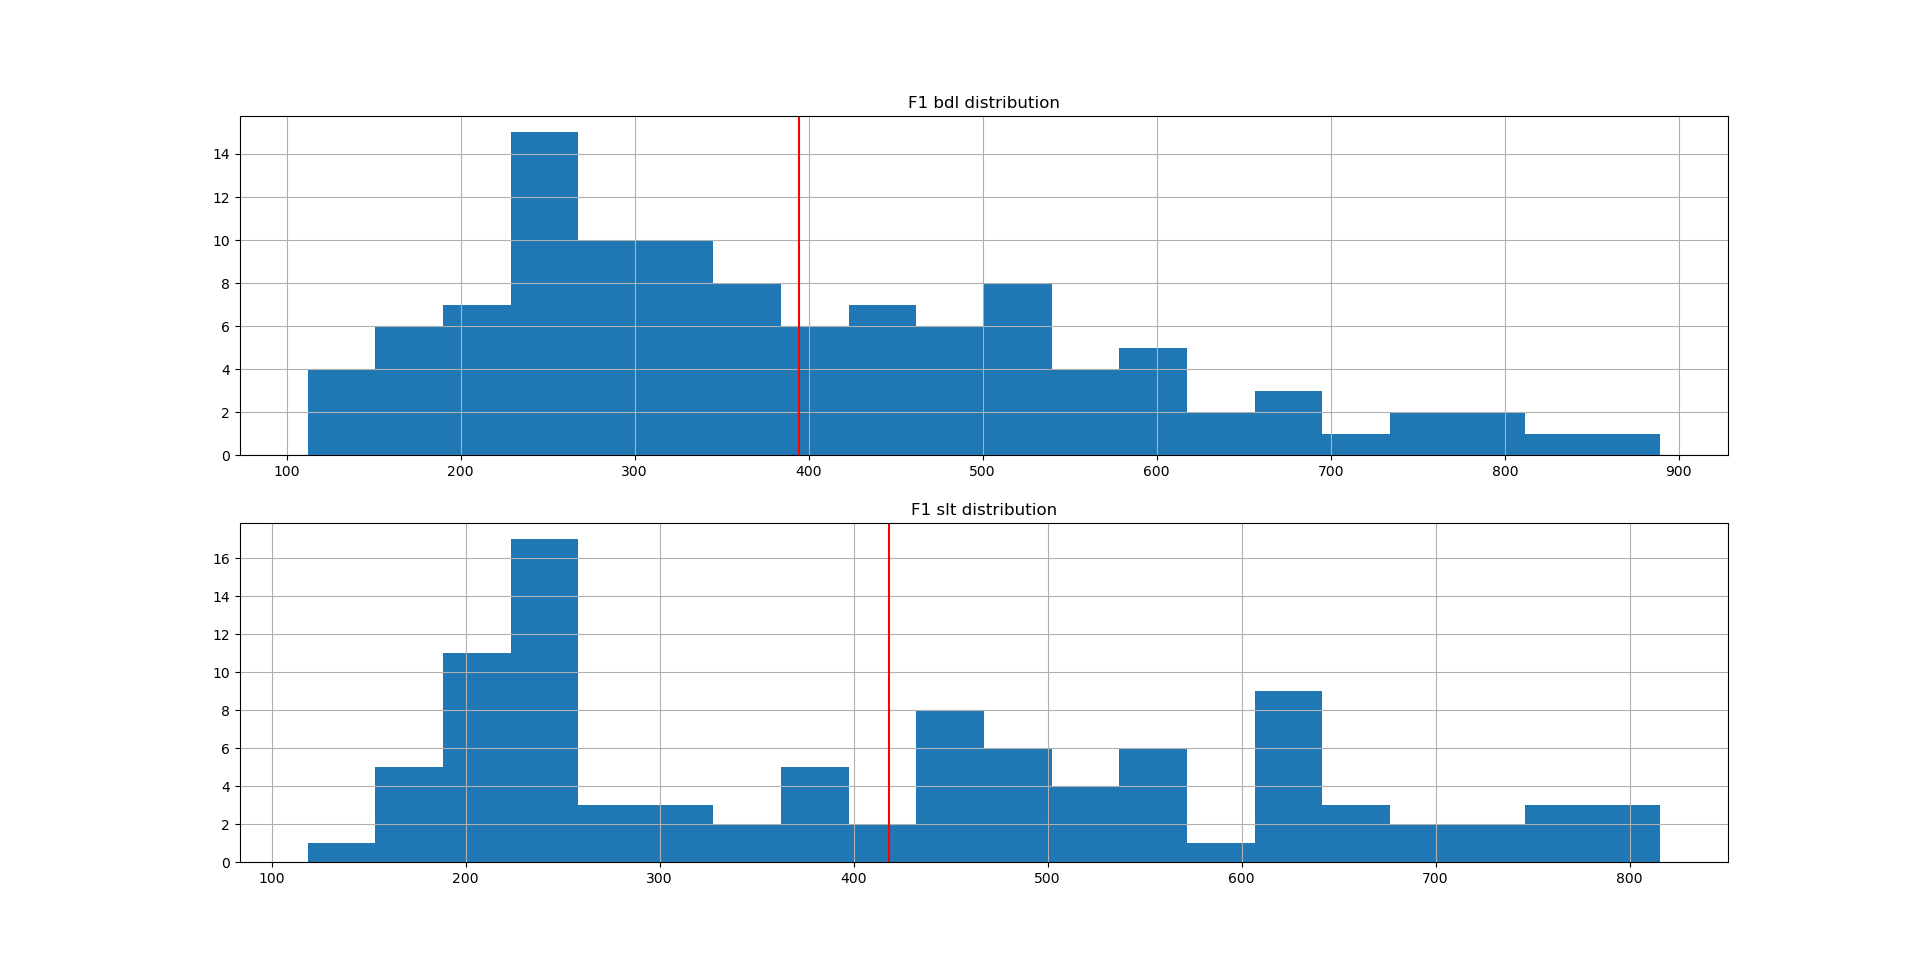
\includegraphics[scale=0.35]{figures/F1_distr_a0006.png}}
	\caption{fichier a0006.wav} 
\end{figure}
\begin{figure}[H]
	\centering
	{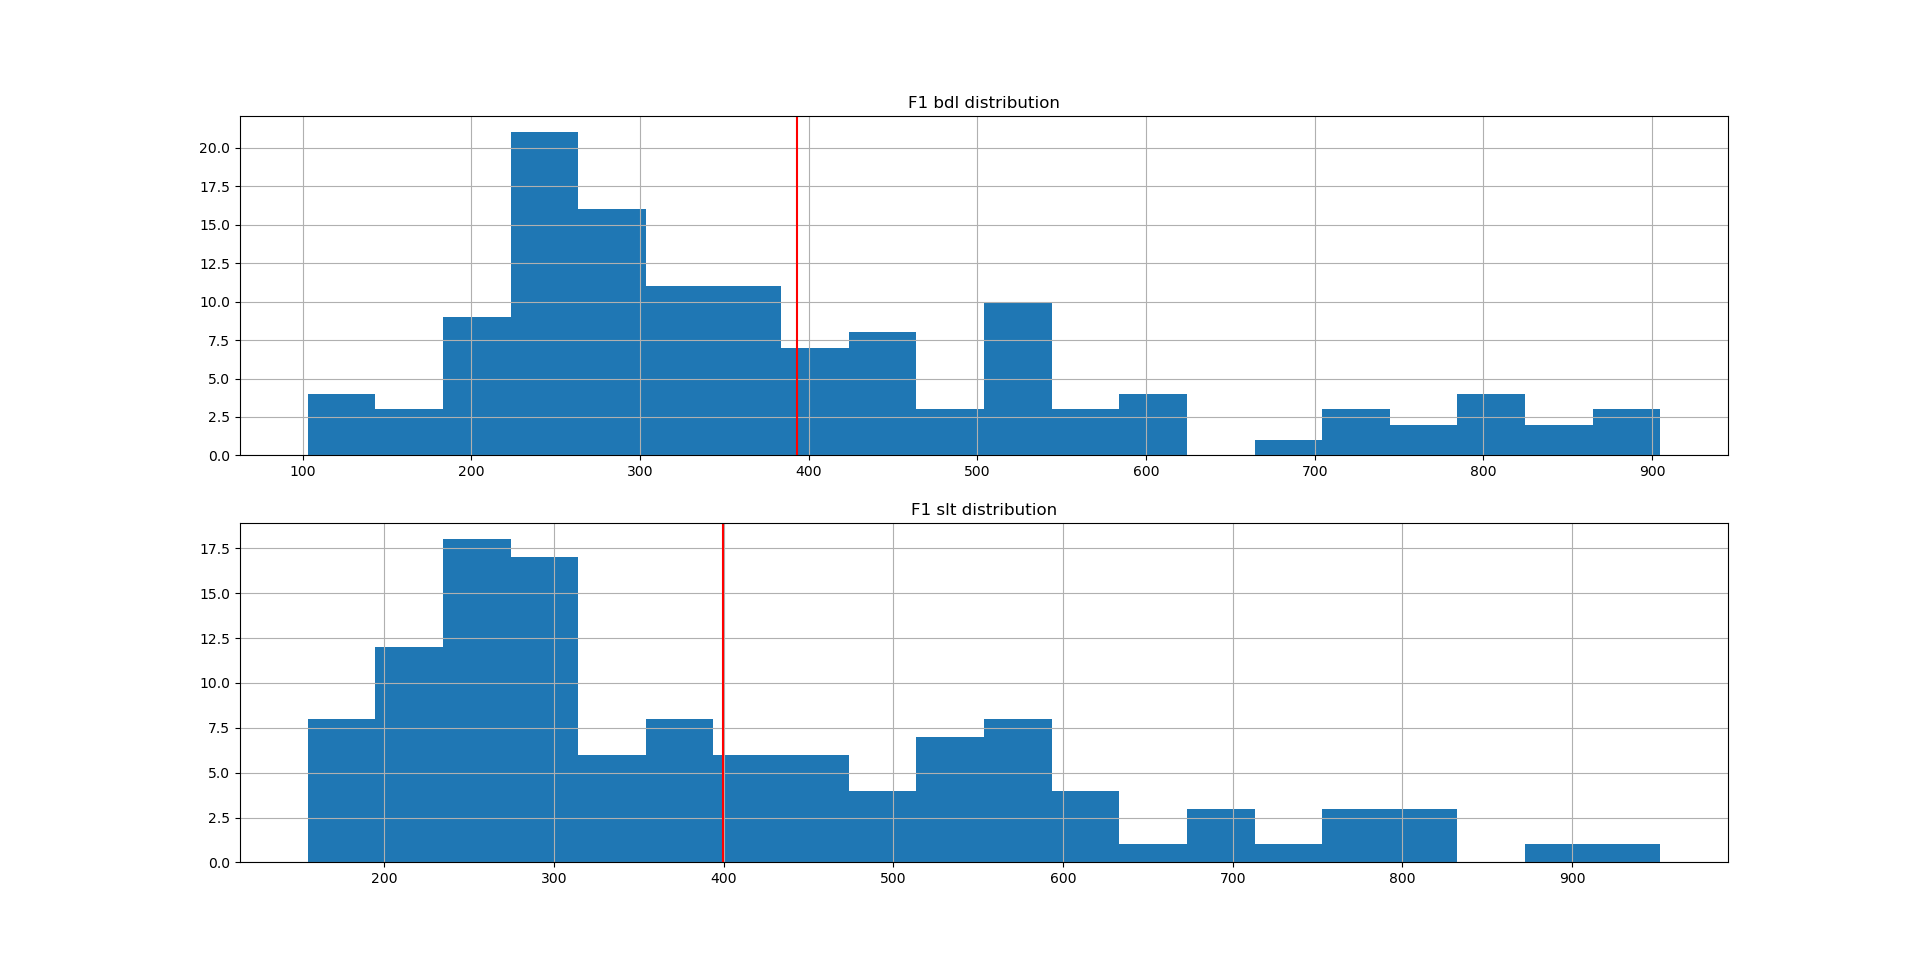
\includegraphics[scale=0.35]{figures/F1_distr_a0392.png}}
	\caption{fichier a0392.wav} 
\end{figure}
\begin{figure}[H]
	{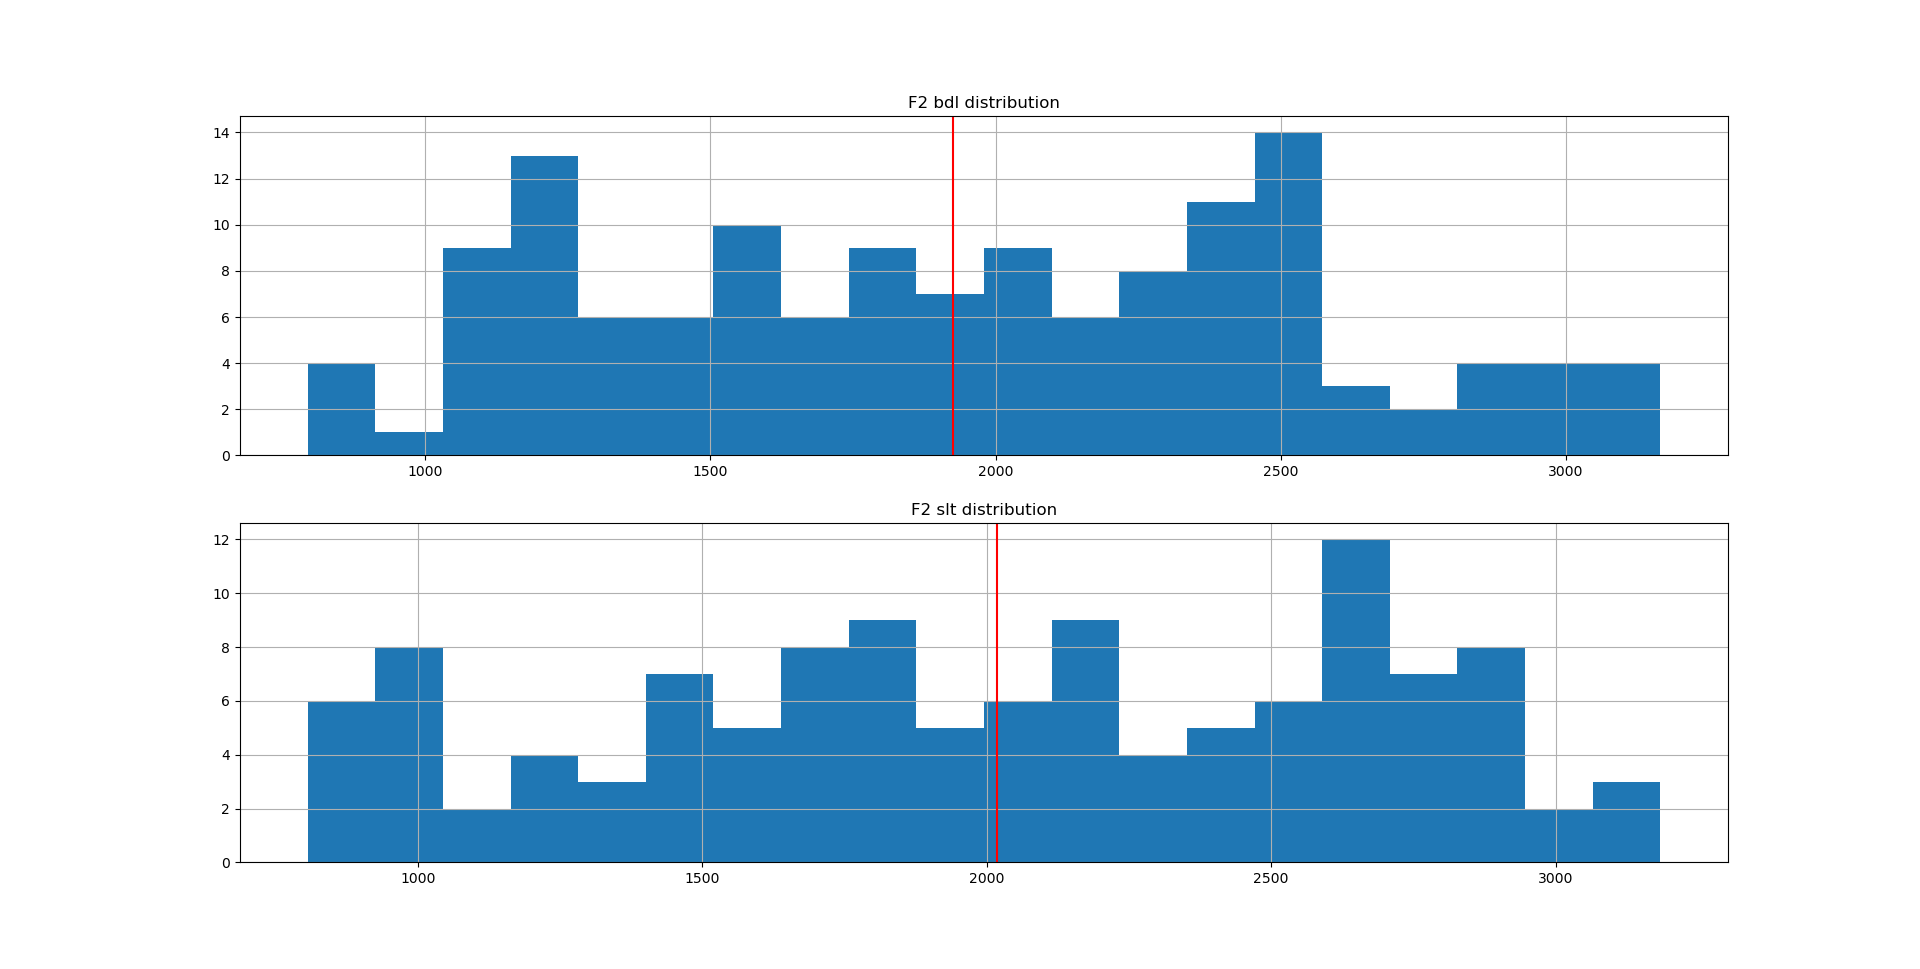
\includegraphics[scale=0.35]{figures/F2_distr_a347.png}}
	\caption{fichier a0347.wav} 
\end{figure}
\begin{figure}[H]
	\centering
	{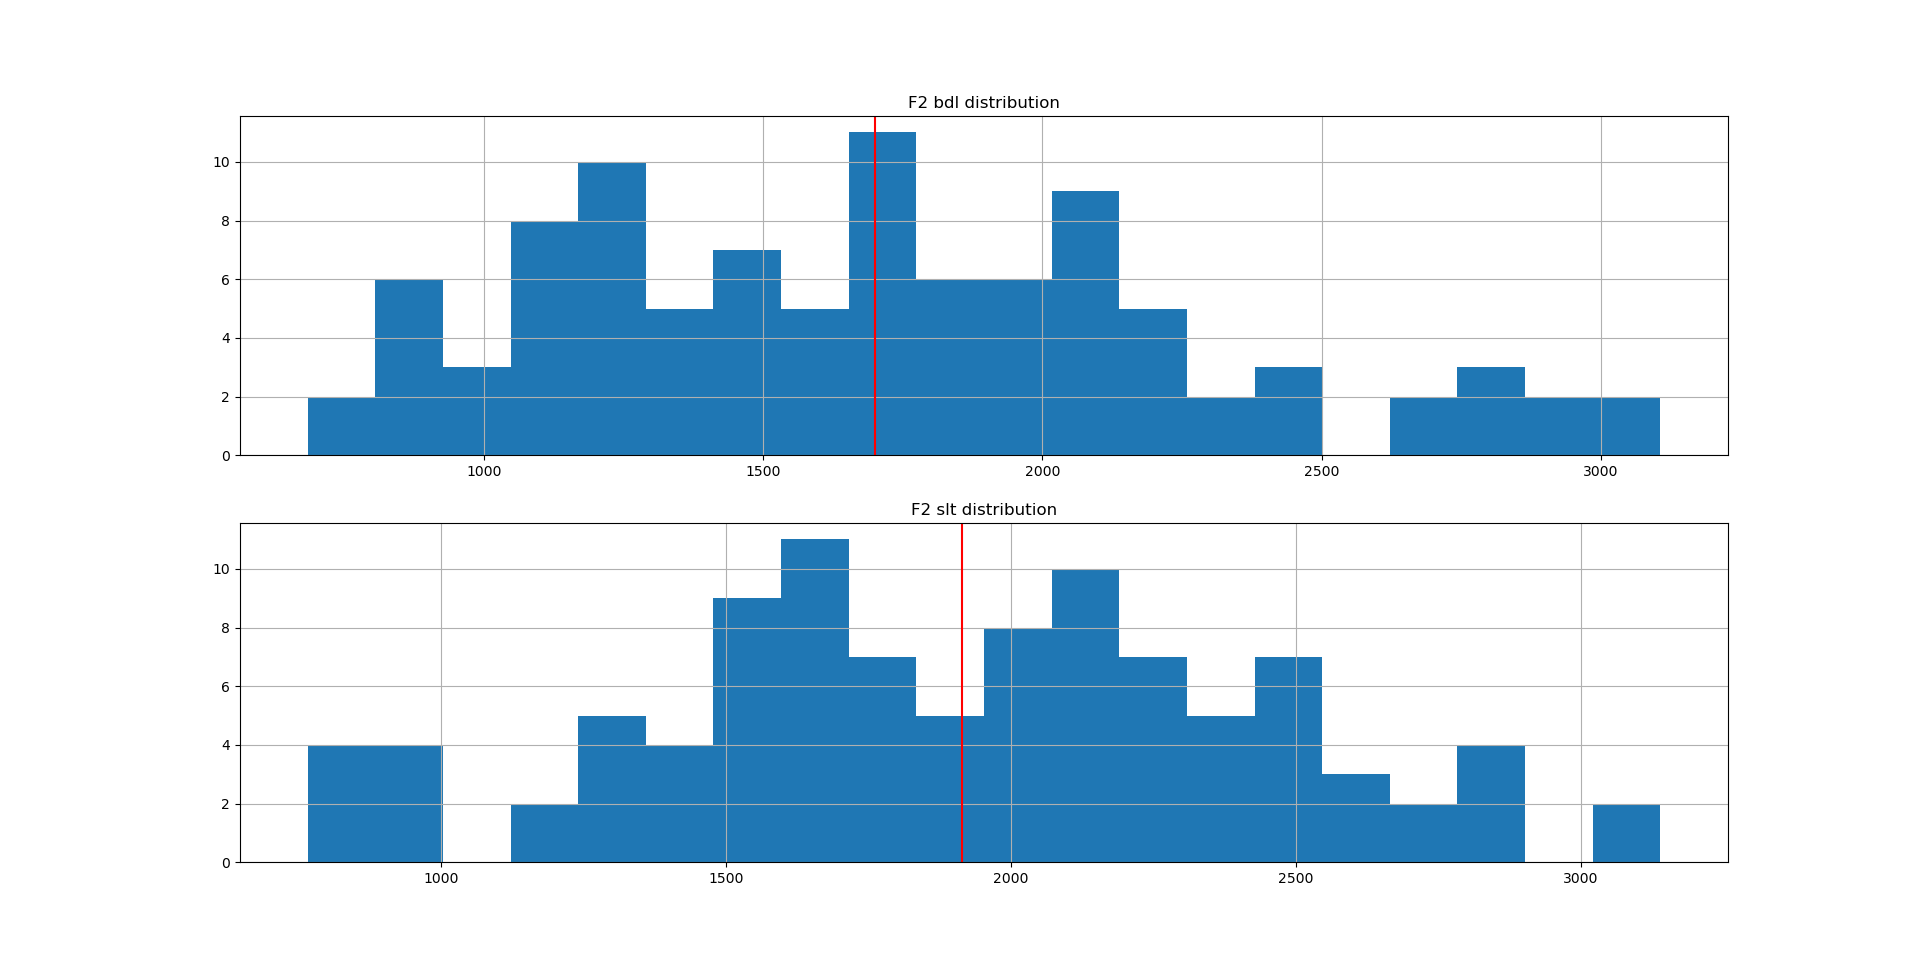
\includegraphics[scale=0.35]{figures/F2_distr_a494.png}}
	\caption{fichier a0494.wav} 
\end{figure}
{\subsection*{2.4 MFCCs}}
\addcontentsline{toc}{section}{2.4 MFCCs}
Les MFCCs représentent les activitées du conduit vocal durant la production de paroles. Afin de les extraire de nos fichiers audio, on a créé l'algorithme compute\_mfcc() prenant un fichier audio comme paramètre. Celui va d'abord extraire le signal et le normaliser. Puis, il va le faire passer par un filtre pass-haut et le diviser en frames de chacune 25ms. Sur chacune de ses frames, une fenêtre de Hamming va être appliquée. Ensuite, on va calculer le spectre de puissance du signal en utilisant l'équation donnée dans l'explication du projet. On changera l'échelle du spectre avec le "Mel\-Filter Bank". Comme les coefficients sont très corrélés, on leur applique une transformée en cosinus discrète, ce qui nous permettra d'avoir les MFCCs, mais on ne prendra que les 13 premiers.
Malheureusement, malgré nos tests, nous avons pas pu trouver une façon de les utiliser pour différencier SLT et BDL.
	
\newpage
{\section*{3. Systèmes basés sur des règles}}
	\addcontentsline{toc}{chapter}{3. Systèmes basés sur des règles}
Nous avons élaboré trois systèmes différents pour effectuer la classification homme/femme. Les trois systèmes fonctionnent de la même manière, ils doivent recevoir en paramètre un chemin menant vers un dossier qui contient au minimum 5 fichiers audio contenant des enregistrements de voix d'une même personne. Le système se charge d'appeler les méthodes pour en extraire les différentes caractéristiques et retourne le résultat, c'est à dire s'il détermine que c'est une femme ou un homme. Afin de tester la précision des systèmes, nous les avons exécuté 10 fois en leur donnant des fichiers des speakers BDL (homme), RMS (homme), SLT (femme) et CMS (femme). Nous avons récupérés son nombre de bonnes classifications et en avons calculé son rapport avec le nombre total de classifications. Plus précisément, nous avons calculé la précision métrique de chaque système sur base d'enregistrements de BDL, RMS, SLT et CMS.

{\subsection*{3.1 Système 01}}
\addcontentsline{toc}{section}{3.1 Système 01}
Le système numéro 1 est implémenté dans la fonction system\_01() et utilise les fréquences fondamentales calculées à partir des deux méthodes décrites ci-dessus ainsi que le formant 1. Nous avons commencé par simplement implémenter les règles définies pour BDL (homme) et SLT (femme) et nous les avons donc extrapolées pour déterminer si il s'agit d'un homme ou d'une femme. Nous avons ensuite affinés les valeurs afin d'améliorer la précision du système. Voici la précision du système : \\
\begin{center}
	\begin{tabular}{|c|c|c|c|c|}
		\hline
		Globale & BDL & SLT & RMS & CMS \\
		\hline
		70\% & 90\% & 90\% & 100\% & 0\% \\
		\hline
		\end{tabular}
\end{center}
Les résultats du système sont bons pour BDL, SLT et RMS mais nul pour CMS souvent en raison du F1.
{\subsection*{3.2 Système 02}}
\addcontentsline{toc}{section}{3.2 Système 02}
Le système numéro 2 est implémenté dans la fonction system\_02() et utilise les fréquences fondamentales calculées à partir des deux méthodes décrites ci-dessus ainsi que le formant 1. Ce système a pour but d'améliorer les performances du système précédent. Pour ce faire, nous avons imaginé attribuer des poids aux différentes caractéristiques. Lorsqu'une caractéristique rentre dans une classe (homme ou femme), alors la probabilité que les fichiers soient de cette classe augmente du poids attribué à cette caractéristique. A la fin, le système regarde quelle probabilité est supérieur à 50\% pour effectuer son choix. Nous avons attribué des poids de 0.4 pour les deux fréquences fondamentales et 0.2 pour le formant 1. Voici la précision du système : \\
\begin{center}
	\begin{tabular}{|c|c|c|c|c|}
		\hline
		Globale & BDL & SLT & RMS & CMS \\
		\hline
		100\% & 100\% & 100\% & 100\% & 100\% \\
		\hline
	\end{tabular}
\end{center}
Le système dispose de très bonnes performances pour BDL, SLT, RMS et CMS. Cependant, son choix se fait majoritairement via le calcul de la fréquence fondamentale. Nous nous questionnons donc sur sa précision lorsqu'il sera confronté à des sujets dont la fréquence fondamentale ne se situe pas dans la moyenne définie. Ce système est cependant celui qui dispose de la meilleur précisions pour les sujets étudiés dans le cadre de ce projet.

{\subsection*{3.3 Système 03}}
\addcontentsline{toc}{section}{3.3 Système 03}
Le système numéro 3 est implémenté dans la fonction system\_03() et utilise les fréquences fondamentales calculées à partir des deux méthodes décrites ci-dessus ainsi que le formant 1 et le formant 2. Le système fonctionne globalement comme le système 1. Il utilise néanmoins le formant 2 en plus et les valeurs utilisées dans les structure conditionnelles ont été affinés. Voici la précision du système : \\
\begin{center}
	\begin{tabular}{|c|c|c|c|c|}
		\hline
		Globale & BDL & SLT & RMS & CMS \\
		\hline
		92.5\% & 80\% & 90\% & 100\% & 100\% \\
		\hline
	\end{tabular}
\end{center}
Les résultats du système sont bons pour BDL, SLT, RMS et CMS.
{\section*{4. Machine learning}}
\addcontentsline{toc}{chapter}{4. Machine learning}
N'ayant jamais fait de machine learning auparavant, nous avons suivi un tutoriel trouvé en ligne que nous avons adapté au projet. \\
Ce tutoriel nous a montré comment utiliser un réseau neuronale implémentant la classification binaire. La classification binaire nous a parue parfaite pour notre problème étant donné que nous n'avons que 2 possibilités de genre : Homme ou Femme. Tout le code de la partie Machine Learning se trouve dans le fichier ml\_utils.py\\
Pour utiliser ce modèle, nous devons lui donner des features en entrée. Ces features permettront au modèle de prendre une décision quant-au genre de la personne parlant dans le fichier audio. Ces features sont au nombre de 4, nous avons pris "autocorrelation pitch", "cepstrum pitch", "formant 1" et "formant 2", ces features sont calculées dans la fonction analyse\_ml(path, firstAudioName) où path est le chemin d'accès au dossier contenant les fichiers audio en .wav et firstAudioName est le nom du fichier a analyser. Une fois ces features calculées pour l'audio, nous ajoutons un label à cet audio, le label dans notre cas est le sexe de la personne qui parle et équivaut à (Homme = 1 | Femme = 0). Nous répétons l'opération pour tous les fichiers des dossiers bdl\_a, bdl\_b, slt\_a ainsi que slt\_b et plaçons tout dans un fichier CSV grâce à la fonction create\_TrainingCSV(). Ce fichier sera le fichier d'entrainement de notre modèle.
En répétant cette manipulation avec les dossiers rms\_a, rms\_b, cms\_a ainsi que cms\_b en passant par la fonction create\_TestCSV() nous créons le fichier de test de notre modèle, ce fichier permettra de tester la validité de la classification de notre modèle. Pour créer notre modèle, nous devons charger les 2 fichiers CSV créés précédement, le fichier d'entrainement (training.csv) et le fichier de test (test.csv). Pour passer les features au modèle nous allons enlever les dernière colonnes des fichiers qui stockent le résultat attendu et les sauvegarder dans des variables (y\_train et y\_test) pour comparer le résultat du modèle plus tard.
Nous allons ensuite instancier un "scaler" pour normaliser nos features d'entrées pour les données d'entrainement et les données de test. Nous fixons le nombre d'EPOCHS (nombre de fois que nous faisons passer le jeux de données d'entrainement au modèle) à 10 car suite à plusieurs essaies, nous avons remarqué que 10 était suffisant et raisonnable. Le BATCH\_SIZE est fixé à 64, ainsi nous envoyons des "paquets" de 64 lignes du CSV de test au modèle lorsqu'il s'entraine. Le dernier BATCH envoyé est inférieur ou égal à 64.
Le LEARNING\_RATE est fixé à 0,001 comme dans le tutoriel. Nous créons ensuite notre "BinaryClassification" modèle en l'instanciant. Le modèle s'entraine ensuite, il effectue une boucle qui lui permet d'optimiser ses WEIGHTs (poids entre les noeuds) et ses BIAS (poids des noeuds) à chaque itération en vérifiant le taux d'erreur qu'il fait. Le taux d'erreur est calculé en comparant la prédiction du vrai label du jeu de test. Une fois le modèle entrainé, il faut savoir le sauvegarder et le charger pour pouvoir l'utiliser, nous utilisons donc la fonction save\_BinaryClassificationModel(model, scaler) pour sauver notre modèle et le scaler, la fonction prend en paramètre le modèle a sauvegarder ainsi que le scaler lié à ce modèle. Pour charger le modèle nous utilisons la fonction load\_BinaryClassificationModel(pathModel, pathScaler) qui retourne le modèle ainsi que le scaler lié au modèle. La fonction prend en paramètres le chemin d'accès au modèle ainsi que le chemin d'accès au scaler.
Pour utiliser le modèle que nous avons entrainé, il suffit d'utiliser la fonction useModel(model, scaler, inputs), avec en paramètre le modèle a utiliser, le scaler associé et une list ([..., ..., ..., ...]) contenant les 4 features d'entrée du modèle. Le modèle prédira si c'est un homme ou une femme en sortie. Le modèle a une efficacité de 100\%, cette manière de faire est plus efficace qu'en essayant plusieurs poids pour chaque feature "à la main" car les poids sont optimisé par le modèle. Celui donne directement la combinaison optimale afin d'optimiser la précision de la classification.\\
Voici le lien du tutoriel sur lequel notre implémentation de la classification binaire s'est basée : \\
\noindent
\url{https://towardsdatascience.com/pytorch-tabular-binary-classification-a0368da5bb89}
\end{document}


